\documentclass{beamer}
\usepackage[nosetup]{evan}
\usepackage{slides}

\newcommand{\stack}[6]{ % read left side, then stack from top to bottom, then right side
    \begin{center}
        \resizebox{8cm}{!}{%
            \begin{tikzpicture}[scale=0.6]
                \draw[draw=none] (-3,-4) -- (6,-4) -- (6,2) -- (-3,2) -- cycle;
                \draw[thick] (-2,0) -- (1,0) -- (1,-3) -- (2,-3) -- (2,0) -- (5,0);
                \node at (3.5,.5) {$#6$};
                \node at (1.5,-2.4) {$#5$};
                \node at (1.5,-1.7) {$#4$};
                \node at (1.5,-1.0) {$#3$};
                \node at (1.5,-.3) {$#2$};
                \node at (-0.5,.5) {$#1$};
            \end{tikzpicture}
        }
    \end{center}
}

\newcommand{\invisstack}{
    \begin{center}
        \resizebox{8cm}{!}{%
            \begin{tikzpicture}[scale=0.6]
                \draw[draw=none] (-3,-4) -- (6,-4) -- (6,2) -- (-3,2) -- cycle;
            \end{tikzpicture}
        }
    \end{center}
}

\newcommand{\bijection}{
    \begin{center}
    \begin{tikzpicture}[scale=0.9, transform shape,
        concept/.style={draw, align=center, rectangle, rounded corners=3pt, text width=2.2cm, font = \small, inner sep = 4pt},
        connection/.style={<->, >=stealth, thick}
    ]
        \uncover<+->{
            \node[concept] (sortable) at (-4.8,0)
                {$s^2$-sortable of $S_n'$};
            \node[concept] (antistandard) at (-1.6,0)
                {\textcolor{asytcolor}{antistandard composition tableaux, width $\le 2$}};
            \draw[connection] (sortable) --
                node[midway, above=2pt] {(1)} (antistandard);
        }
        \uncover<+->{
            \node[concept] (standard) at (1.6,0)
                {\textcolor{sytcolor}{standard Young tableaux, width $\le 3$}};
            \draw[connection] (antistandard) --
                node[midway, above=2pt] {(2)} (standard);
        }
        \uncover<+->{
            \node[concept] (motzkin) at (4.8,0)
                {Motzkin numbers};
            \draw[connection] (standard) --
                node[midway, above=2pt] {(3)} (motzkin);
        }
    \end{tikzpicture}
    \end{center}
    \blfootnote{\tiny Figure generated with AI assistance.}
}

\newcommand{\thm}{
    \begin{theorem}[L.\ 2026]
        \# of $s^2$-sortable permutations in $S_n'$ is $n$th Motzkin number.
    \end{theorem}
}

\newcommand{\arw}{\longleftrightarrow}

\newcommand{\RED}[1]{\textcolor{red}{\mathbf #1}}
\newcommand{\GRN}[1]{\textcolor{YellowGreen}{\mathbf #1}}
\definecolor{asytcolor}{RGB}{0,114,178}
\definecolor{sytcolor}{RGB}{213,94,0}

\author[Michael Luo]{\texorpdfstring{Michael Luo \\ Research Science Institute \\ Mentor: Ryota Inagaki}{}}
\date{August 2026}

\begin{document}

\title{Resolving a Conjecture on Stack-Sorting}
\frame{\titlepage}
\title{Penguins}
\frame{\titlepage}

\begin{asydef}
size(12cm);

picture body;
pen border = black+1.2;
path outline = (0,0)..(0.5,-0.1)..(0.9,0)..(0.9,0)..(1,0.7)
..(0.85,1.3)..(0.4,1.32)..(0.13,1.1)..(0.12,1.08)--(0.12,1.08)..(0.03,0.4)
..(0,0.1)--(0,0.02)--(0,0)..cycle;
filldraw(body, (0.8,0.7)--(1.15,0.35)--(0.85,0.4)--cycle, rgb("#90a0b0"), border);
filldraw(body, outline, rgb("#90a0b0"), border);
filldraw(body, subpath(outline, 0.2, 6.6)
    --(0.25,0.9)..(0.25,0.7)--(0.44,0.52)--(0.27,0.45)
    ..(0.2,0.22)..(0.15,0.1)..cycle,
rgb("#f4f4f4"), border);
filldraw(body, ellipse((0.32,-0.075), 0.12, 0.07), orange, border);
filldraw(body, ellipse((0.72,-0.07), 0.12, 0.07), orange, border);
draw(body, (0.51,1.07)..(0.59,1.09)..(0.66,1.07), black+1.5);
draw(body, (0.78,1.07)..(0.86,1.09)..(0.94,1.07), black+1.5);
filldraw(body, (0.7,0.98)--(0.89,0.92)--(0.68,0.89)--cycle, yellow, border);

picture body1;
picture body2;
picture body3;
picture body4;
add(body1,shift(0.5 - 0.1,0.18)*xscale(-0.9)*yscale(0.9)*body);
add(body2,shift(0.5 - 0.03,0.22)*xscale(-1.0)*yscale(1.1)*body);
add(body3,shift(0.5 + 0.03,0.24)*xscale(-1.1)*yscale(1.3)*body);
add(body4,shift(0.5 + 0.1,0.27)*xscale(-1.2)*yscale(1.5)*body);

// Numeral sizes are proportional to the penguins' vertical scales.
label(body1, "$\mathsf{1}$", (-0.11 - 0.1,0.6), fontsize(12pt)+red);
label(body2, "$\mathsf{2}$", (-0.15 - 0.03,0.8), fontsize(14.67pt)+red);
label(body3, "$\mathsf{3}$", (-0.25 + 0.03,0.9), fontsize(17.33pt)+red);
label(body4, "$\mathsf{4}$", (-0.32 + 0.1,1.0), fontsize(20pt)+red);

pen boxborder = deepgreen+2;

picture background;
draw(background, (-7,0)--(-1,0)--(-1,-5)--(1,-5)--(1,0)--(7,0), boxborder);
draw(background, (-8,-5)--(8,-5)--(8,3)--(-8,3)--cycle, invisible);

picture twoholebackground;
draw(twoholebackground,
    (-11.75,0)--(-5.25,0)--(-5.25,-5)--(-3.25,-5)--(-3.25,0)
    --(3.25,0)--(3.25,-5)--(5.25,-5)--(5.25,0)--(11.75,0),
    boxborder);
draw(twoholebackground, (-12.5,-5)--(12.5,-5)--(12.5,3)--(-12.5,3)--cycle, invisible);

void placeontwohole(real offset) {
    picture shifted;
    add(shifted, shift(offset,0)*currentpicture);
    erase();
    add(shifted);
    add(twoholebackground);
}
\end{asydef}

% Render each overlay image once, then reuse the cached box in its Beamer overlay.
\newcommand{\showpenguin}[1]{%
    \raisebox{0pt}[171.079pt][0pt]{\makebox[\textwidth][c]{\usebox{#1}}}%
}
\newsavebox{\penguinFirstOne}
\newsavebox{\penguinFirstTwo}
\newsavebox{\penguinFirstThree}
\newsavebox{\penguinFirstFour}
\newsavebox{\penguinFirstFive}
\newsavebox{\penguinFirstSix}
\newsavebox{\penguinFirstSeven}
\newsavebox{\penguinFirstEight}
\newsavebox{\penguinFirstNine}
\newsavebox{\penguinSecondOne}
\newsavebox{\penguinSecondTwo}
\newsavebox{\penguinSecondThree}
\newsavebox{\penguinSecondFour}
\newsavebox{\penguinSecondFive}
\newsavebox{\penguinSecondSix}
\newsavebox{\penguinSecondSeven}
\newsavebox{\penguinSecondEight}
\newsavebox{\penguinSecondNine}

\begin{lrbox}{\penguinFirstOne}
\begin{asy}
add(shift(2,0)*body3);
add(shift(3.5,0)*body1);
add(shift(5,0)*body4);
add(shift(6.5,0)*body2);
placeontwohole(4.25);
\end{asy}
\end{lrbox}

\begin{lrbox}{\penguinFirstTwo}
\begin{asy}
add(shift(0,-5)*body3);
add(shift(3.5,0)*body1);
add(shift(5,0)*body4);
add(shift(6.5,0)*body2);
placeontwohole(4.25);
\end{asy}
\end{lrbox}

\begin{lrbox}{\penguinFirstThree}
\begin{asy}
add(shift(0,-5)*body3);
add(shift(0,-5 + 1.95)*body1);
add(shift(5,0)*body4);
add(shift(6.5,0)*body2);
placeontwohole(4.25);
\end{asy}
\end{lrbox}

\begin{lrbox}{\penguinFirstFour}
\begin{asy}
add(shift(0,-5)*body3);
add(shift(-6.5,0)*body1);
add(shift(5,0)*body4);
add(shift(6.5,0)*body2);
placeontwohole(4.25);
\end{asy}
\end{lrbox}

\begin{lrbox}{\penguinFirstFive}
\begin{asy}
add(shift(-5,0)*body3);
add(shift(-6.5,0)*body1);
add(shift(5,0)*body4);
add(shift(6.5,0)*body2);
placeontwohole(4.25);
\end{asy}
\end{lrbox}

\begin{lrbox}{\penguinFirstSix}
\begin{asy}
add(shift(-5,0)*body3);
add(shift(-6.5,0)*body1);
add(shift(0,-5)*body4);
add(shift(6.5,0)*body2);
placeontwohole(4.25);
\end{asy}
\end{lrbox}

\begin{lrbox}{\penguinFirstSeven}
\begin{asy}
add(shift(-5,0)*body3);
add(shift(-6.5,0)*body1);
add(shift(0,-5)*body4);
add(shift(0,-5 + 2.15)*body2);
placeontwohole(4.25);
\end{asy}
\end{lrbox}

\begin{lrbox}{\penguinFirstEight}
\begin{asy}
add(shift(-5,0)*body3);
add(shift(-6.5,0)*body1);
add(shift(0,-5)*body4);
add(shift(-3.5,0)*body2);
placeontwohole(4.25);
\end{asy}
\end{lrbox}

\begin{lrbox}{\penguinFirstNine}
\begin{asy}
add(shift(-5,0)*body3);
add(shift(-6.5,0)*body1);
add(shift(-2,0)*body4);
add(shift(-3.5,0)*body2);
placeontwohole(4.25);
\end{asy}
\end{lrbox}

\begin{lrbox}{\penguinSecondOne}
\begin{asy}
add(shift(2,0)*body1);
add(shift(3.5,0)*body3);
add(shift(5,0)*body2);
add(shift(6.5,0)*body4);
placeontwohole(-4.25);
\end{asy}
\end{lrbox}

\begin{lrbox}{\penguinSecondTwo}
\begin{asy}
add(shift(0,-5)*body1);
add(shift(3.5,0)*body3);
add(shift(5,0)*body2);
add(shift(6.5,0)*body4);
placeontwohole(-4.25);
\end{asy}
\end{lrbox}

\begin{lrbox}{\penguinSecondThree}
\begin{asy}
add(shift(-6.5,0)*body1);
add(shift(3.5,0)*body3);
add(shift(5,0)*body2);
add(shift(6.5,0)*body4);
placeontwohole(-4.25);
\end{asy}
\end{lrbox}

\begin{lrbox}{\penguinSecondFour}
\begin{asy}
add(shift(-6.5,0)*body1);
add(shift(0,-5)*body3);
add(shift(5,0)*body2);
add(shift(6.5,0)*body4);
placeontwohole(-4.25);
\end{asy}
\end{lrbox}

\begin{lrbox}{\penguinSecondFive}
\begin{asy}
add(shift(-6.5,0)*body1);
add(shift(0,-5)*body3);
add(shift(0,-5 + 1.95)*body2);
add(shift(6.5,0)*body4);
placeontwohole(-4.25);
\end{asy}
\end{lrbox}

\begin{lrbox}{\penguinSecondSix}
\begin{asy}
add(shift(-6.5,0)*body1);
add(shift(0,-5)*body3);
add(shift(-5,0)*body2);
add(shift(6.5,0)*body4);
placeontwohole(-4.25);
\end{asy}
\end{lrbox}

\begin{lrbox}{\penguinSecondSeven}
\begin{asy}
add(shift(-6.5,0)*body1);
add(shift(-3.5,0)*body3);
add(shift(-5,0)*body2);
add(shift(6.5,0)*body4);
placeontwohole(-4.25);
\end{asy}
\end{lrbox}

\begin{lrbox}{\penguinSecondEight}
\begin{asy}
add(shift(-6.5,0)*body1);
add(shift(-3.5,0)*body3);
add(shift(-5,0)*body2);
add(shift(0,-5)*body4);
placeontwohole(-4.25);
\end{asy}
\end{lrbox}

\begin{lrbox}{\penguinSecondNine}
\begin{asy}
add(shift(-6.5,0)*body1);
add(shift(-3.5,0)*body3);
add(shift(-5,0)*body2);
add(shift(-2,0)*body4);
placeontwohole(-4.25);
\end{asy}
\end{lrbox}

\begin{frame}
\uncover<3->{Penguins are
\begin{itemize}
    \ii \textbf{Impatient:} small penguins will always jump on big penguins
    \uncover<5->{\ii \textbf{Considerate:} big penguins won't jump on small penguins}
\end{itemize}}
\begin{center}
\only<1>{\showpenguin{\penguinFirstOne}}%
\only<2-3>{\showpenguin{\penguinFirstTwo}}%
\only<4-5>{\showpenguin{\penguinFirstThree}}%
\only<6>{\showpenguin{\penguinFirstFour}}%
\only<7>{\showpenguin{\penguinFirstFive}}%
\only<8>{\showpenguin{\penguinFirstSix}}%
\only<9>{\showpenguin{\penguinFirstSeven}}%
\only<10>{\showpenguin{\penguinFirstEight}}%
\only<11>{\showpenguin{\penguinFirstNine}}%
\only<12>{\showpenguin{\penguinSecondTwo}}%
\only<13>{\showpenguin{\penguinSecondThree}}%
\only<14>{\showpenguin{\penguinSecondFour}}%
\only<15>{\showpenguin{\penguinSecondFive}}%
\only<16>{\showpenguin{\penguinSecondSix}}%
\only<17>{\showpenguin{\penguinSecondSeven}}%
\only<18>{\showpenguin{\penguinSecondEight}}%
\only<19>{\showpenguin{\penguinSecondNine}}
\end{center}
\blfootnote{\tiny Penguins by Evan Chen, used with permission. Figure generated with AI assistance.}
\end{frame}

\begin{frame}[fragile]
    \begin{center}
    \begin{asy}
    size(7cm);
    add(shift(1.5,0)*body3);
    add(shift(3.0,0)*body1);
    add(shift(4.5,0)*body4);
    add(shift(6.0,0)*body2);

    draw((4.25,0)--(4.25,-0.8), black+linewidth(1pt), Arrow(size=6), BeginBar(size=6));
    label("$s$", (4.25,-0.4), E);

    add(shift(1.5,-3)*body1);
    add(shift(3.0,-3)*body3);
    add(shift(4.5,-3)*body2);
    add(shift(6.0,-3)*body4);

    draw((4.25,-3)--(4.25,-3.8), black+linewidth(1pt), Arrow(size=6), BeginBar(size=6));
    label("$s$", (4.25,-3.4), E);

    add(shift(1.5,-6)*body1);
    add(shift(3.0,-6)*body2);
    add(shift(4.5,-6)*body3);
    add(shift(6.0,-6)*body4);
    \end{asy}
    \end{center}
    In notation: $s(3142) = 1324$, $s(1324) = 1234$
    \blfootnote{\tiny Figure generated with AI assistance.}
\end{frame}

\begin{frame}
    \frametitle{Main result}
    \[S_3 = \{123,132,213,231,312,321\}\]
    \pause
    \begin{itemize}
        \ii \# of $s$-sortable in $S_n$: $\frac1{n + 1}\binom{2n}n$ (Knuth 1968).
        \pit \# of $s^2$-sortable in $S_n$: $\frac2{(n + 1)(2n + 1)}\binom{3n}n$ (Zeilberger 1992).
    \end{itemize}
    \pause
    \medskip
    \[S_3' = \{123\GRN0,132\GRN0,213\GRN0,231\GRN0,312\GRN0,321\GRN0\}\]
    \pause
    \begin{itemize}
        \ii \# of $s$-sortable in $S_n'$: $1$.
        \pit \# of $s^2$-sortable in $S_n'$: ??
    \end{itemize}
    \pause
    \thm
\end{frame}

\begin{frame}[fragile]
    $n$th Motzkin counts:

    \only<1>{
    Ways to draw any \# of disjoint chords connecting $n$ points on a circle
    \medskip

    \begin{tikzpicture}[x=0.72cm,y=0.72cm,
        chord/.style={red!80!black, line width=1.5pt},
        dot/.style={circle, fill=black, inner sep=1.25pt}]
        \tikzset{motzkin circle/.pic={
            \filldraw[fill=gray!0, draw=gray!70, line width=0.7pt]
                (0,0) circle[radius=0.72];
        }}
        \tikzset{motzkin dots/.pic={
            \node[dot] at (-0.51, 0.51) {};
            \node[dot] at ( 0.51, 0.51) {};
            \node[dot] at ( 0.51,-0.51) {};
            \node[dot] at (-0.51,-0.51) {};
        }}

        \node[anchor=west] at (0, 2.2) {$0$ chords:};
        \node[anchor=west] at (0, 0)   {$1$ chord:};
        \node[anchor=west] at (0,-2.2) {$2$ chords:};

        % No chords.
        \pic at (3.25,2.2) {motzkin circle};
        \pic at (3.25,2.2) {motzkin dots};

        % The six ways to choose one chord.
        \foreach \x in {3.25,4.95,6.65,8.35,10.05,11.75}
            \pic at (\x,0) {motzkin circle};
        \draw[chord,shift={(3.25,0)}]  (-0.51, 0.51)--( 0.51, 0.51);
        \draw[chord,shift={(4.95,0)}]  (-0.51, 0.51)--( 0.51,-0.51);
        \draw[chord,shift={(6.65,0)}]  (-0.51, 0.51)--(-0.51,-0.51);
        \draw[chord,shift={(8.35,0)}]  ( 0.51, 0.51)--( 0.51,-0.51);
        \draw[chord,shift={(10.05,0)}] ( 0.51, 0.51)--(-0.51,-0.51);
        \draw[chord,shift={(11.75,0)}] ( 0.51,-0.51)--(-0.51,-0.51);
        \foreach \x in {3.25,4.95,6.65,8.35,10.05,11.75}
            \pic at (\x,0) {motzkin dots};

        % The two noncrossing perfect matchings.
        \pic at (3.25,-2.2) {motzkin circle};
        \pic at (4.95,-2.2) {motzkin circle};
        \draw[chord,shift={(3.25,-2.2)}]
            (-0.51,0.51)--(0.51,0.51)
            (0.51,-0.51)--(-0.51,-0.51);
        \draw[chord,shift={(4.95,-2.2)}]
            (-0.51,0.51)--(-0.51,-0.51)
            (0.51,0.51)--(0.51,-0.51);
        \pic at (3.25,-2.2) {motzkin dots};
        \pic at (4.95,-2.2) {motzkin dots};
    \end{tikzpicture}
    \blfootnote{\tiny Figure generated with AI assistance.}
    }
    \only<2>{
    Number of \textcolor{sytcolor}{standard Young tableaux with width $\le 3$} (Regev 1981)
    \[
    % https://q.uiver.app/#q=WzAsMyxbMCwyXSxbMiwwXSxbMCwwXSxbMiwwLCJcXHRleHR7aW5jcmVhc2luZ30iLDJdLFsyLDEsIlxcdGV4dHtpbmNyZWFzaW5nfSJdXQ==
    \begin{tikzcd}[ampersand replacement=\&]
        {} \&\& {} \\
        \\
        {}
        \arrow["{\text{increasing}}", from=1-1, to=1-3]
        \arrow["{\text{increasing}}"', from=1-1, to=3-1]
    \end{tikzcd}
    {\color{sytcolor}\begin{matrix}
        \tab{1 \\ 2 \\ 3 \\ 4} & \tab{1 & 2 \\ 3 \\ 4} & \tab{1 & 3 \\ 2 \\ 4} \vspace{0.5cm} \\
        \tab{1 & 4 \\ 2 \\ 3} & \tab{1 & 2 \\ 3 & 4} & \tab{1 & 3 \\ 2 & 4} \vspace{0.5cm} \\
        \tab{1 & 3 & 4 \\ 2} & \tab{1 & 2 & 4 \\ 3} & \tab{1 & 2 & 3 \\ 4}
    \end{matrix}}\]

    }
    \only<3>{
    \begin{figure}
        \centering
        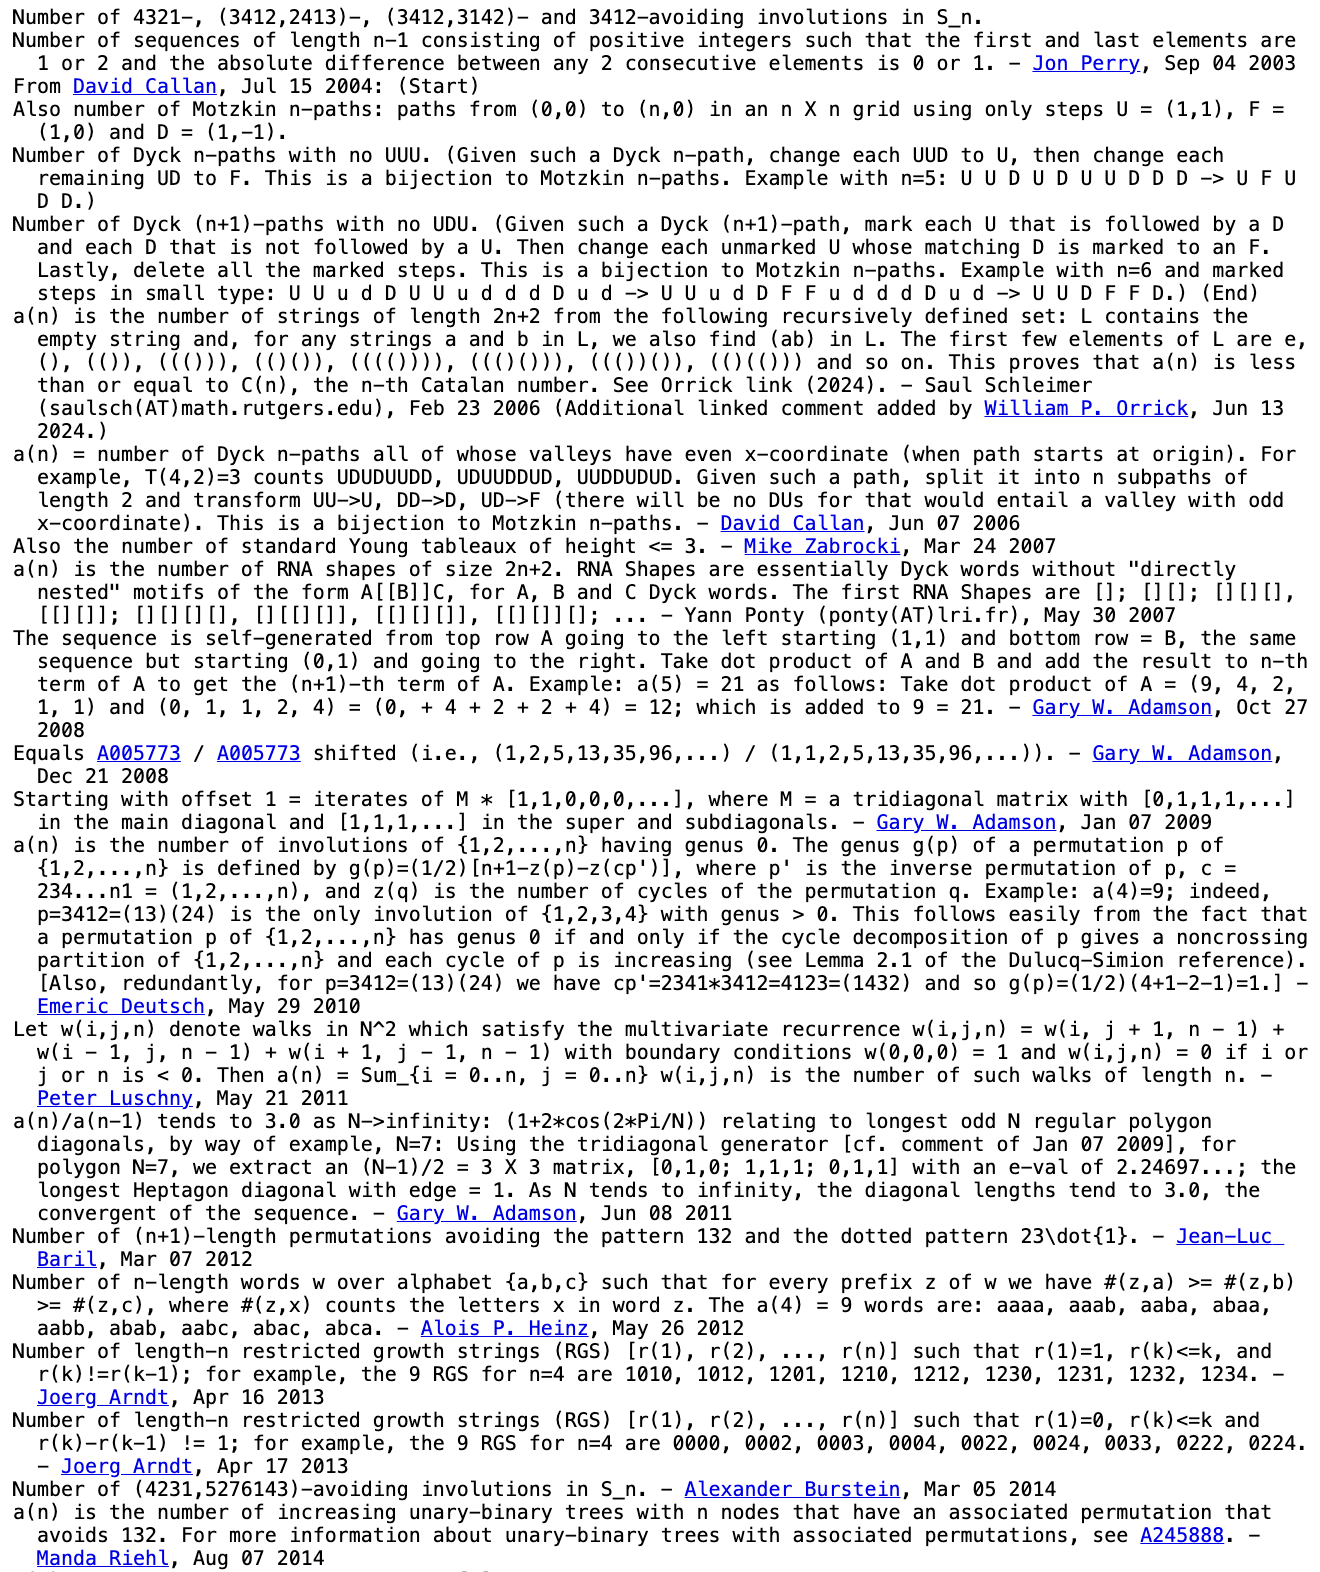
\includegraphics[width=0.49\linewidth]{Images/oeis1.png}
        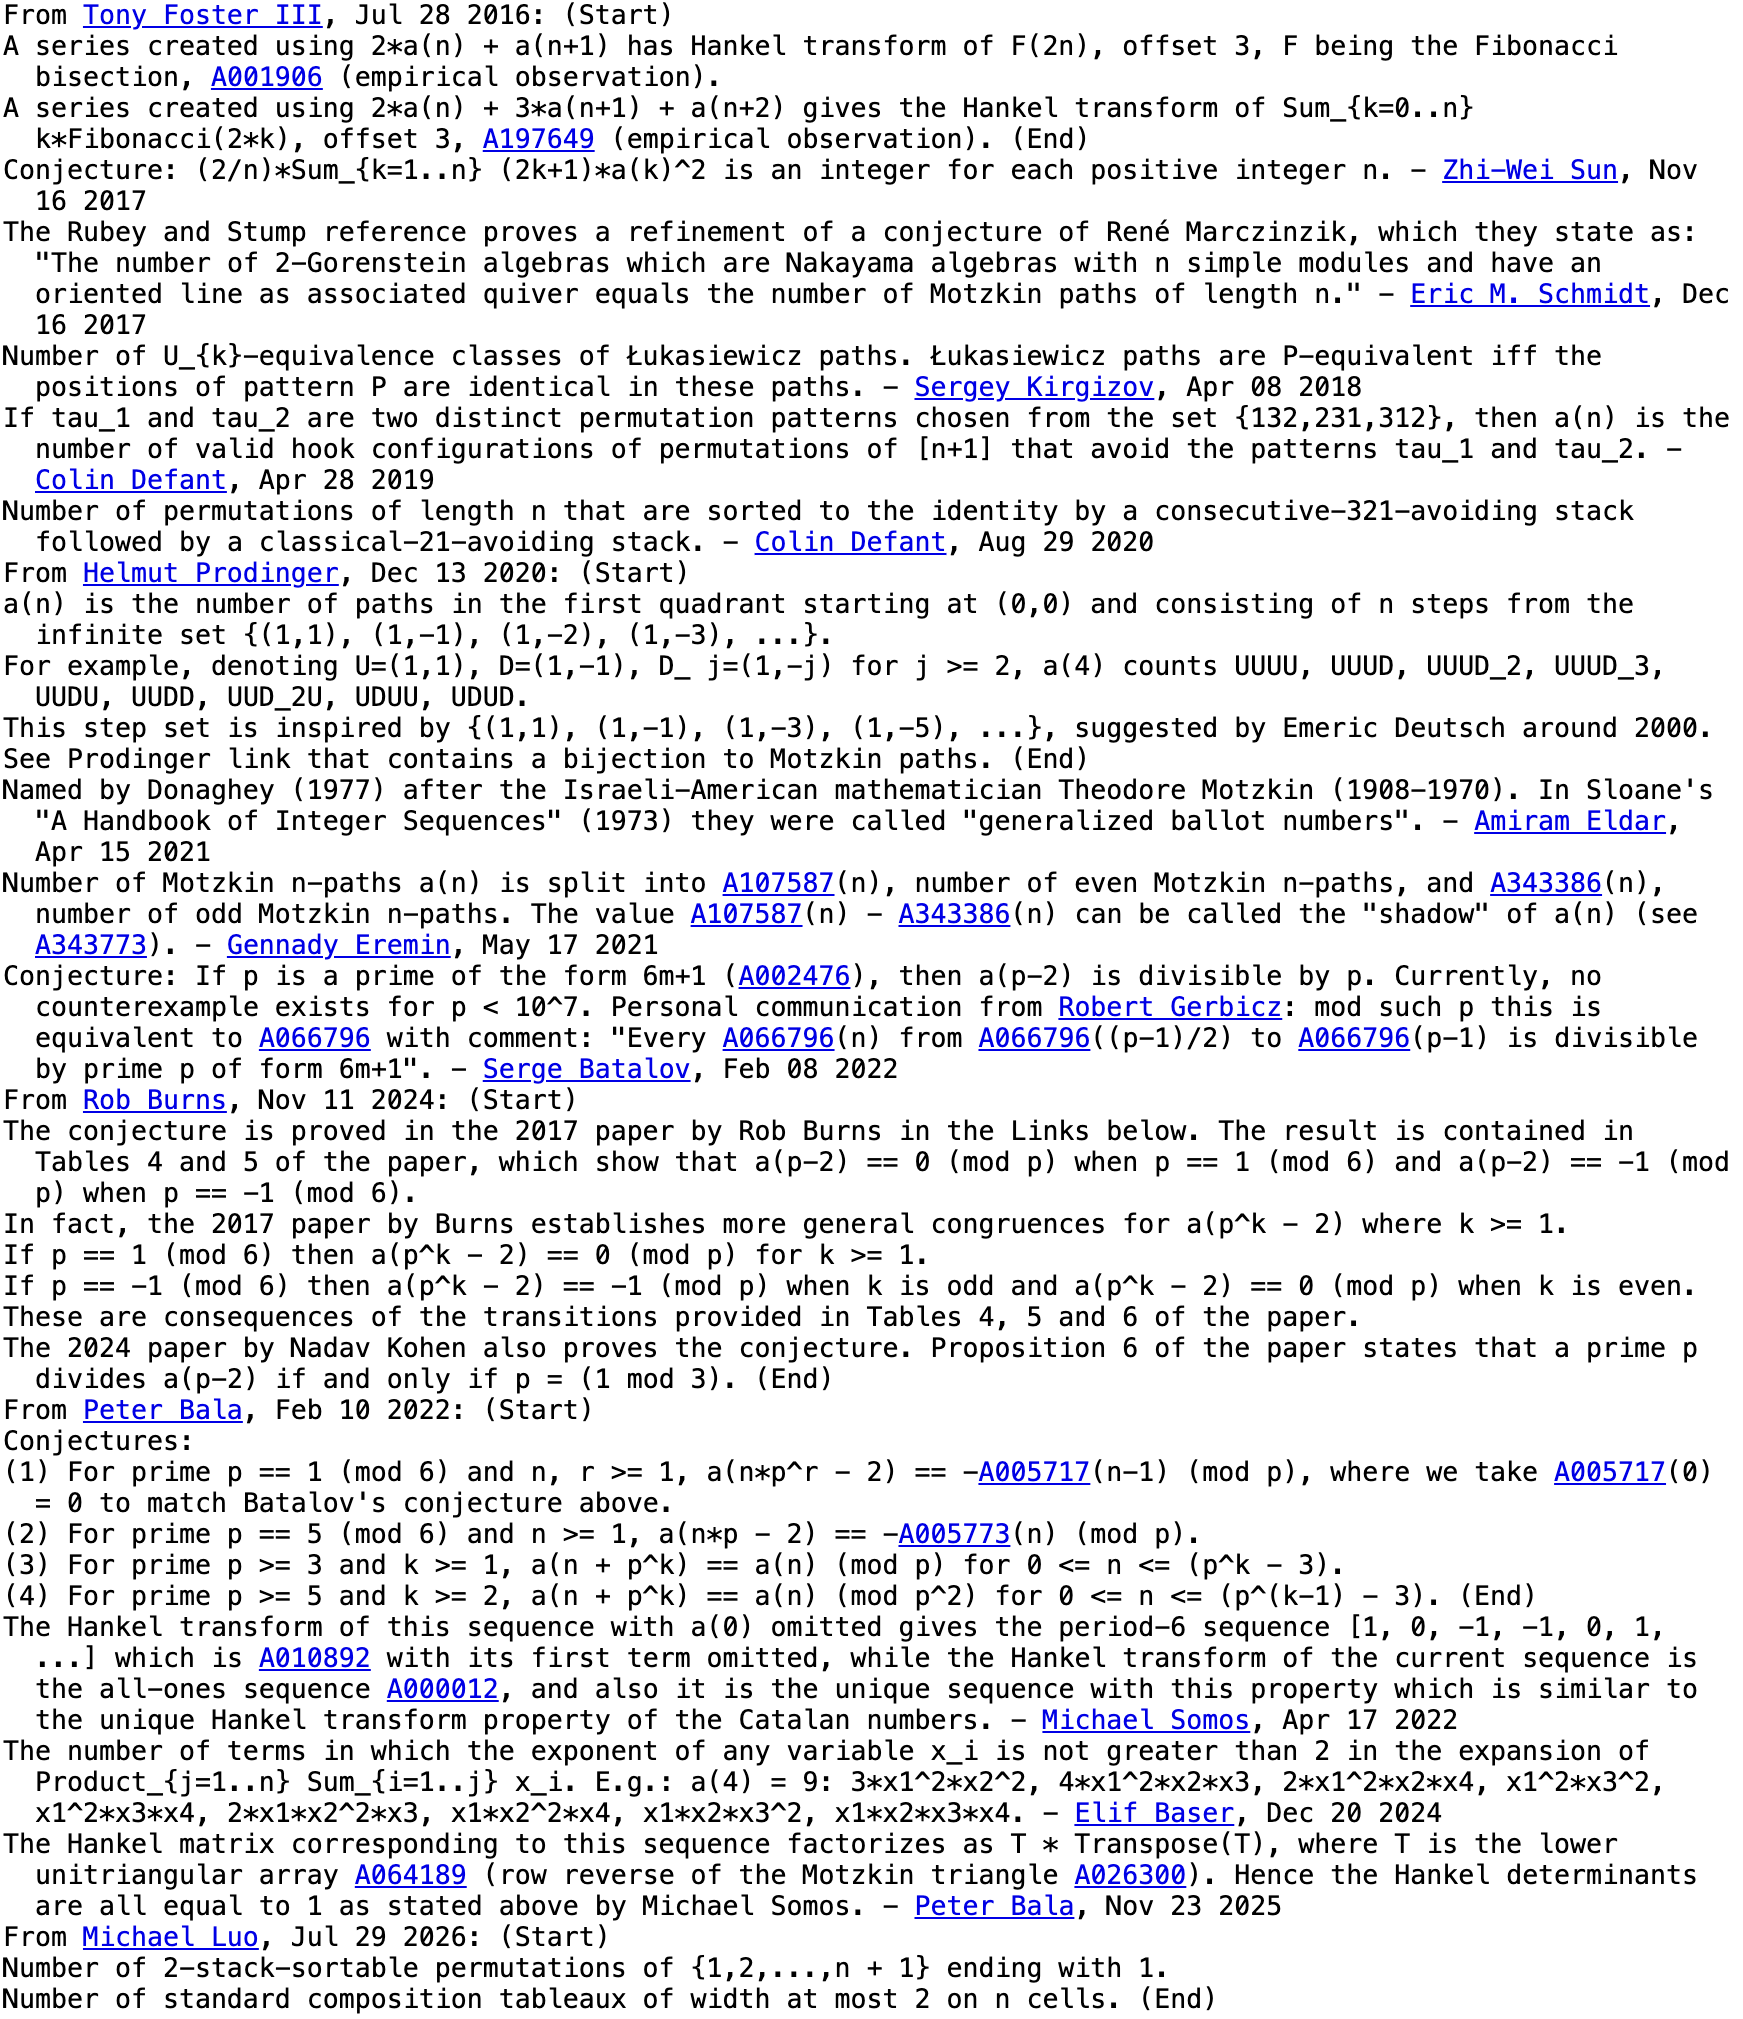
\includegraphics[width=0.49\linewidth]{Images/oeis2.png}
    \end{figure}
    \blfootnote{\tiny Online Encyclopedia of Integer Sequences, August 5, 2026}
    }
\end{frame}

\begin{frame}[t]
    \frametitle{Proof idea}
    \thm
    Idea: matching! \pause

    \bijection
\end{frame}

\begin{frame}[t]
    \vspace*{0pt}
    \begin{lemma}[Chen-L.-Zhang 2025, Zhang 2026]
        Take $\pi \in S_n'$ and apply $s$ repeatedly. Then
        \begin{itemize}
            \ii each time, the \textcolor{red}{right-to-left maxima} of the part before $\GRN 0$ go after $\GRN 0$ and
            \ii the part after $\GRN 0$ is always sorted.
        \end{itemize}
    \end{lemma}
    \begin{overlayarea}{\textwidth}{6cm}
    \only<1-3,49>{\LARGE
    \begin{align*}
        \uncover<1-3,49>{4\RED6\RED521\RED3\GRN0 &\xmapsto s 412\GRN 0\RED3\RED5\RED6} \\
        \uncover<2-3,49>{\RED41\RED2\GRN0356 &\xmapsto s 1\GRN0\RED23\RED456} \\
        \uncover<3,49>{\RED1\GRN023456 &\xmapsto s \GRN0\RED123456}
    \end{align*}
    }
    \only<4-18>{{\LARGE\[4\RED6\RED521\RED3\GRN0 \xmapsto s 412\GRN 0\RED3\RED5\RED6\]}\vspace{-1.5cm}}%
    \only<4>{\stack{}{}{}{}{}{4\RED6\RED521\RED3\GRN0}}%
    \only<5>{\stack{}{}{}{}{4}{\RED6\RED521\RED3\GRN0}}%
    \only<6>{\stack{4}{}{}{}{}{\RED6\RED521\RED3\GRN0}}%
    \only<7>{\stack{4}{}{}{}{\RED6}{\RED521\RED3\GRN0}}%
    \only<8>{\stack{4}{}{}{\RED5}{\RED6}{21\RED3\GRN0}}%
    \only<9>{\stack{4}{}{2}{\RED5}{\RED6}{1\RED3\GRN0}}%
    \only<10>{\stack{4}{1}{2}{\RED5}{\RED6}{\RED3\GRN0}}%
    \only<11>{\stack{41}{}{2}{\RED5}{\RED6}{\RED3\GRN0}}%
    \only<12>{\stack{412}{}{}{\RED5}{\RED6}{\RED3\GRN0}}%
    \only<13>{\stack{412}{}{\RED3}{\RED5}{\RED6}{\GRN0}}%
    \only<14>{\stack{412}{\GRN0}{\RED3}{\RED5}{\RED6}{}}%
    \only<15>{\stack{412\GRN0}{}{\RED3}{\RED5}{\RED6}{}}%
    \only<16>{\stack{412\GRN0\RED3}{}{}{\RED5}{\RED6}{}}%
    \only<17>{\stack{412\GRN0\RED3\RED5}{}{}{}{\RED6}{}}%
    \only<18>{\stack{412\GRN0\RED3\RED5\RED6}{}{}{}{}{}}%
    \only<19-33>{{\LARGE\[\RED41\RED2\GRN0356 \xmapsto s 1\GRN0\RED23\RED456\]}\vspace{-1.5cm}}%
    \only<19>{\stack{}{}{}{}{}{\RED41\RED2\GRN0356}}%
    \only<20>{\stack{}{}{}{}{\RED4}{1\RED2\GRN0356}}%
    \only<21>{\stack{}{}{}{1}{\RED4}{\RED2\GRN0356}}%
    \only<22>{\stack{1}{}{}{}{\RED4}{\RED2\GRN0356}}%
    \only<23>{\stack{1}{}{}{\RED2}{\RED4}{\GRN0356}}%
    \only<24>{\stack{1}{}{\GRN0}{\RED2}{\RED4}{356}}%
    \only<25>{\stack{1\GRN0}{}{}{\RED2}{\RED4}{356}}%
    \only<26>{\stack{1\GRN0\RED2}{}{}{}{\RED4}{356}}%
    \only<27>{\stack{1\GRN0\RED2}{}{}{3}{\RED4}{56}}%
    \only<28>{\stack{1\GRN0\RED23}{}{}{}{\RED4}{56}}%
    \only<29>{\stack{1\GRN0\RED23\RED4}{}{}{}{}{56}}%
    \only<30>{\stack{1\GRN0\RED23\RED4}{}{}{}{5}{6}}%
    \only<31>{\stack{1\GRN0\RED23\RED45}{}{}{}{}{6}}%
    \only<32>{\stack{1\GRN0\RED23\RED45}{}{}{}{6}{}}%
    \only<33>{\stack{1\GRN0\RED23\RED456}{}{}{}{}{}}%
    \only<34-48>{{\LARGE\[\RED1\GRN023456 \xmapsto s \GRN0\RED123456\]}\vspace{-1.5cm}}%
    \only<34>{\stack{}{}{}{}{}{\RED1\GRN023456}}%
    \only<35>{\stack{}{}{}{}{\RED1}{\GRN023456}}%
    \only<36>{\stack{}{}{}{\GRN0}{\RED1}{23456}}%
    \only<37>{\stack{\GRN0}{}{}{}{\RED1}{23456}}%
    \only<38>{\stack{\GRN0\RED1}{}{}{}{}{23456}}%
    \only<39>{\stack{\GRN0\RED1}{}{}{}{2}{3456}}%
    \only<40>{\stack{\GRN0\RED12}{}{}{}{}{3456}}%
    \only<41>{\stack{\GRN0\RED12}{}{}{}{3}{456}}%
    \only<42>{\stack{\GRN0\RED123}{}{}{}{}{456}}%
    \only<43>{\stack{\GRN0\RED123}{}{}{}{4}{56}}%
    \only<44>{\stack{\GRN0\RED1234}{}{}{}{}{56}}%
    \only<45>{\stack{\GRN0\RED1234}{}{}{}{5}{6}}%
    \only<46>{\stack{\GRN0\RED12345}{}{}{}{}{6}}%
    \only<47>{\stack{\GRN0\RED12345}{}{}{}{6}{}}%
    \only<48>{\stack{\GRN0\RED123456}{}{}{}{}{}}%
    \end{overlayarea}
\end{frame}

\begin{frame}
    $\RED3\RED1\GRN0245$ is $s$-sortable since all elements before $0$ are right-to-left maxima
    \begin{center}
        \begin{tikzpicture}[
            scale=0.5,
            vertex/.style={circle, fill, inner sep=1.2pt}
        ]
            \node[vertex, label={[xshift=-6pt, yshift=- 9pt]:{$\RED3$}}] (p1) at (1,3) {};
            \node[vertex, label={[xshift=-6pt, yshift=-12pt]:{$\RED1$}}] (p2) at (2,1) {};
            \node[vertex, label={[xshift= 0pt, yshift=-17pt]:{$\GRN0$}}] (p3) at (3,0) {};
            \node[vertex, label={[xshift= 6pt, yshift=-12pt]:{$2$}}]     (p4) at (4,2) {};
            \node[vertex, label={[xshift= 6pt, yshift=-12pt]:{$4$}}]     (p5) at (5,4) {};
            \node[vertex, label={[xshift= 6pt, yshift=-12pt]:{$5$}}]     (p6) at (6,5) {};

            \draw[thick] (p1) -- (p2) -- (p3) -- (p4) -- (p5) -- (p6);
        \end{tikzpicture}
    \end{center}
    \pause
    $s$-sortable permutations are V-shaped!
    \pause
    Only one $s$-sortable in $S_n'$:
    \begin{center}
        \begin{tikzpicture}[
            scale=0.5,
            vertex/.style={circle, fill, inner sep=1.2pt}
        ]
            \node[vertex, label={[xshift=-6pt, yshift=-12pt]:{$\RED5$}}] (p1) at (1,5) {};
            \node[vertex, label={[xshift=-6pt, yshift=-12pt]:{$\RED4$}}] (p2) at (2,4) {};
            \node[vertex, label={[xshift=-6pt, yshift=-12pt]:{$\RED3$}}] (p3) at (3,3) {};
            \node[vertex, label={[xshift=-6pt, yshift=-12pt]:{$\RED2$}}] (p4) at (4,2) {};
            \node[vertex, label={[xshift=-6pt, yshift=-12pt]:{$\RED1$}}] (p5) at (5,1) {};
            \node[vertex, label={[xshift=-6pt, yshift=-12pt]:{$\GRN0$}}] (p6) at (6,0) {};

            \draw[thick] (p1) -- (p2) -- (p3) -- (p4) -- (p5) -- (p6);
        \end{tikzpicture}
    \end{center}
\end{frame}

\begin{frame}
    If $\pi \in S_n'$ is $s^2$-sortable, $\le 1$ elements between RL-maxima of $\pi$
    \[\begin{matrix}
        \boxed{\text{\LARGE $\RED42\RED3\RED1\GRN0$}} \qquad & \qquad \boxed{\text{\LARGE $\RED421\RED3\GRN0$}} \\
        \text{good} \qquad & \qquad \text{bad}
    \end{matrix}\]
    \vspace{-1cm}
    \only<1>{\invisstack}
    \only<2>{\stack{}{}{}{}{}{\RED421\RED3\GRN0}}
    \only<3>{\stack{}{}{}{}{\RED4}{21\RED3\GRN0}}
    \only<4>{\stack{}{}{}{2}{\RED4}{1\RED3\GRN0}}
    \only<5>{\stack{}{}{1}{2}{\RED4}{\RED3\GRN0}}
    \only<6>{\stack{1}{}{}{2}{\RED4}{\RED3\GRN0}}
    \only<7>{\stack{12}{}{}{}{\RED4}{\RED3\GRN0}}
    \only<8>{\stack{12}{}{}{\RED3}{\RED4}{\GRN0}}
    \only<9>{\stack{12}{}{\GRN0}{\RED3}{\RED4}{}}
    \only<10>{\stack{12\GRN0}{}{}{\RED3}{\RED4}{}}
    \only<11>{\stack{12\GRN0\RED3}{}{}{}{\RED4}{}}
    \only<12>{\stack{12\GRN0\RED3\RED4}{}{}{}{}{}}
\end{frame}

\begin{frame}
    \begin{align*}
        \text{\LARGE$3\RED5\RED41\RED2\GRN0$} \qquad \uncover<2-3>{&\arw \qquad {\color{asytcolor}\begin{ytableau}\RED5 & 3 \\ \RED4 \\ \RED2 & 1\end{ytableau}}} \\
        \text{\LARGE$4\RED8\RED7\RED63\RED51\RED2\GRN0$} \qquad \uncover<2-3>{&\arw \qquad {\color{asytcolor}\begin{ytableau}\RED8 & 4 \\ \RED7 \\ \RED6 \\ \RED5 & 3 \\ \RED2 & 1 \end{ytableau}}}
    \end{align*}
    \pause
    \uncover<3>{\begin{itemize}
        \ii Rows and columns decreasing
        \ii Entries are exactly $\{1,2,\dots,n\}$
        \ii Width at most $2$
    \end{itemize}
    ``Antistandard composition tableaux with width at most $2$''}
\end{frame}

\begin{frame}
    \[\text{$s^2$-sortable of $S_n'$} \arw \text{\textcolor{asytcolor}{antistandard composition tableaux, width $\le 2$}}\]
    \begin{align*}
        43210 &\arw {\color{asytcolor}\tab{4 \\ 3 \\ 2 \\ 1}} &
        34210 &\arw {\color{asytcolor}\tab{4 & 3 \\ 2 \\ 1}} &
        24310 &\arw {\color{asytcolor}\tab{4 & 2 \\ 3 \\ 1}} \\
        14320 &\arw {\color{asytcolor}\tab{4 & 1 \\ 3 \\ 2}} &
        42310 &\arw {\color{asytcolor}\tab{4 \\ 3 & 2 \\ 1}} &
        41320 &\arw {\color{asytcolor}\tab{4 \\ 3 & 1 \\ 2}} \\
        43120 &\arw {\color{asytcolor}\tab{4 \\ 3 \\ 2 & 1}} &
        34120 &\arw {\color{asytcolor}\tab{4 & 3 \\ 2 & 1}} &
        24130 &\arw {\color{asytcolor}\tab{4 & 2 \\ 3 & 1}}
    \end{align*}
\end{frame}

\begin{frame}
    My result:
    \vspace{-0.4cm}
    \begin{multline*}
        \textcolor{asytcolor}{\text{antistandard composition tableaux, width $\le 2$}} \arw \\
        \textcolor{sytcolor}{\text{standard Young tableaux, width $\le 3$}}
    \end{multline*}
    \vspace{-1.4cm}
    \begin{center}
    \begin{tikzpicture}[
        asyt tableau/.style={text=asytcolor, inner sep=2pt},
        syt tableau/.style={text=sytcolor, inner sep=2pt}
    ]
        % Each translucent band groups one vertical column of three tableaux.
        \foreach \x in {-5.85,-1.65,2.55}
            \filldraw[fill=asytcolor, fill opacity=0.18,
                draw=asytcolor, draw opacity=0.35, rounded corners=3pt]
                (\x-0.6,-2.90) rectangle (\x+0.6,3.20);
        \foreach \x in {-3.55,0.65,4.85}
            \filldraw[fill=sytcolor, fill opacity=0.18,
                draw=sytcolor, draw opacity=0.35, rounded corners=3pt]
                (\x-0.87,-2.90) rectangle (\x+0.87,3.20);

        \node[asyt tableau] at (-5.85, 2.00) {$\tab{4 \\ 3 \\ 2 \\ 1}$};
        \node[asyt tableau] at (-5.85, 0)    {$\tab{4 & 1 \\ 3 \\ 2}$};
        \node[asyt tableau] at (-5.85,-2.00) {$\tab{4 \\ 3 \\ 2 & 1}$};
        \node[syt tableau]  at (-3.55, 2.00) {$\tab{1 \\ 2 \\ 3 \\ 4}$};
        \node[syt tableau]  at (-3.55, 0)    {$\tab{1 & 4 \\ 2 \\ 3}$};
        \node[syt tableau]  at (-3.55,-2.00) {$\tab{1 & 3 & 4 \\ 2}$};

        \node[asyt tableau] at (-1.65, 2.00) {$\tab{4 & 3 \\ 2 \\ 1}$};
        \node[asyt tableau] at (-1.65, 0)    {$\tab{4 \\ 3 & 2 \\ 1}$};
        \node[asyt tableau] at (-1.65,-2.00) {$\tab{4 & 3 \\ 2 & 1}$};
        \node[syt tableau]  at ( 0.65, 2.00) {$\tab{1 & 2 \\ 3 \\ 4}$};
        \node[syt tableau]  at ( 0.65, 0)    {$\tab{1 & 2 & 3 \\ 4}$};
        \node[syt tableau]  at ( 0.65,-2.00) {$\tab{1 & 2 \\ 3 & 4}$};

        \node[asyt tableau] at ( 2.55, 2.00) {$\tab{4 & 2 \\ 3 \\ 1}$};
        \node[asyt tableau] at ( 2.55, 0)    {$\tab{4 \\ 3 & 1 \\ 2}$};
        \node[asyt tableau] at ( 2.55,-2.00) {$\tab{4 & 2 \\ 3 & 1}$};
        \node[syt tableau]  at ( 4.85, 2.00) {$\tab{1 & 3 \\ 2 \\ 4}$};
        \node[syt tableau]  at ( 4.85, 0)    {$\tab{1 & 2 & 4 \\ 3}$};
        \node[syt tableau]  at ( 4.85,-2.00) {$\tab{1 & 3 \\ 2 & 4}$};

        \foreach \x in {-4.80,-0.60,3.60}
            \foreach \y in {2.00,0,-2.00}
                \node at (\x,\y) {$\arw$};
    \end{tikzpicture}
    \end{center}
    \blfootnote{\tiny Figure generated with AI assistance.}
\end{frame}

\begin{frame}
    \bijection
    \uncover<4>\thm
\end{frame}

\begin{frame}
    \only<1>{
    $n$th Motzkin counts:
    \begin{figure}
        \centering
        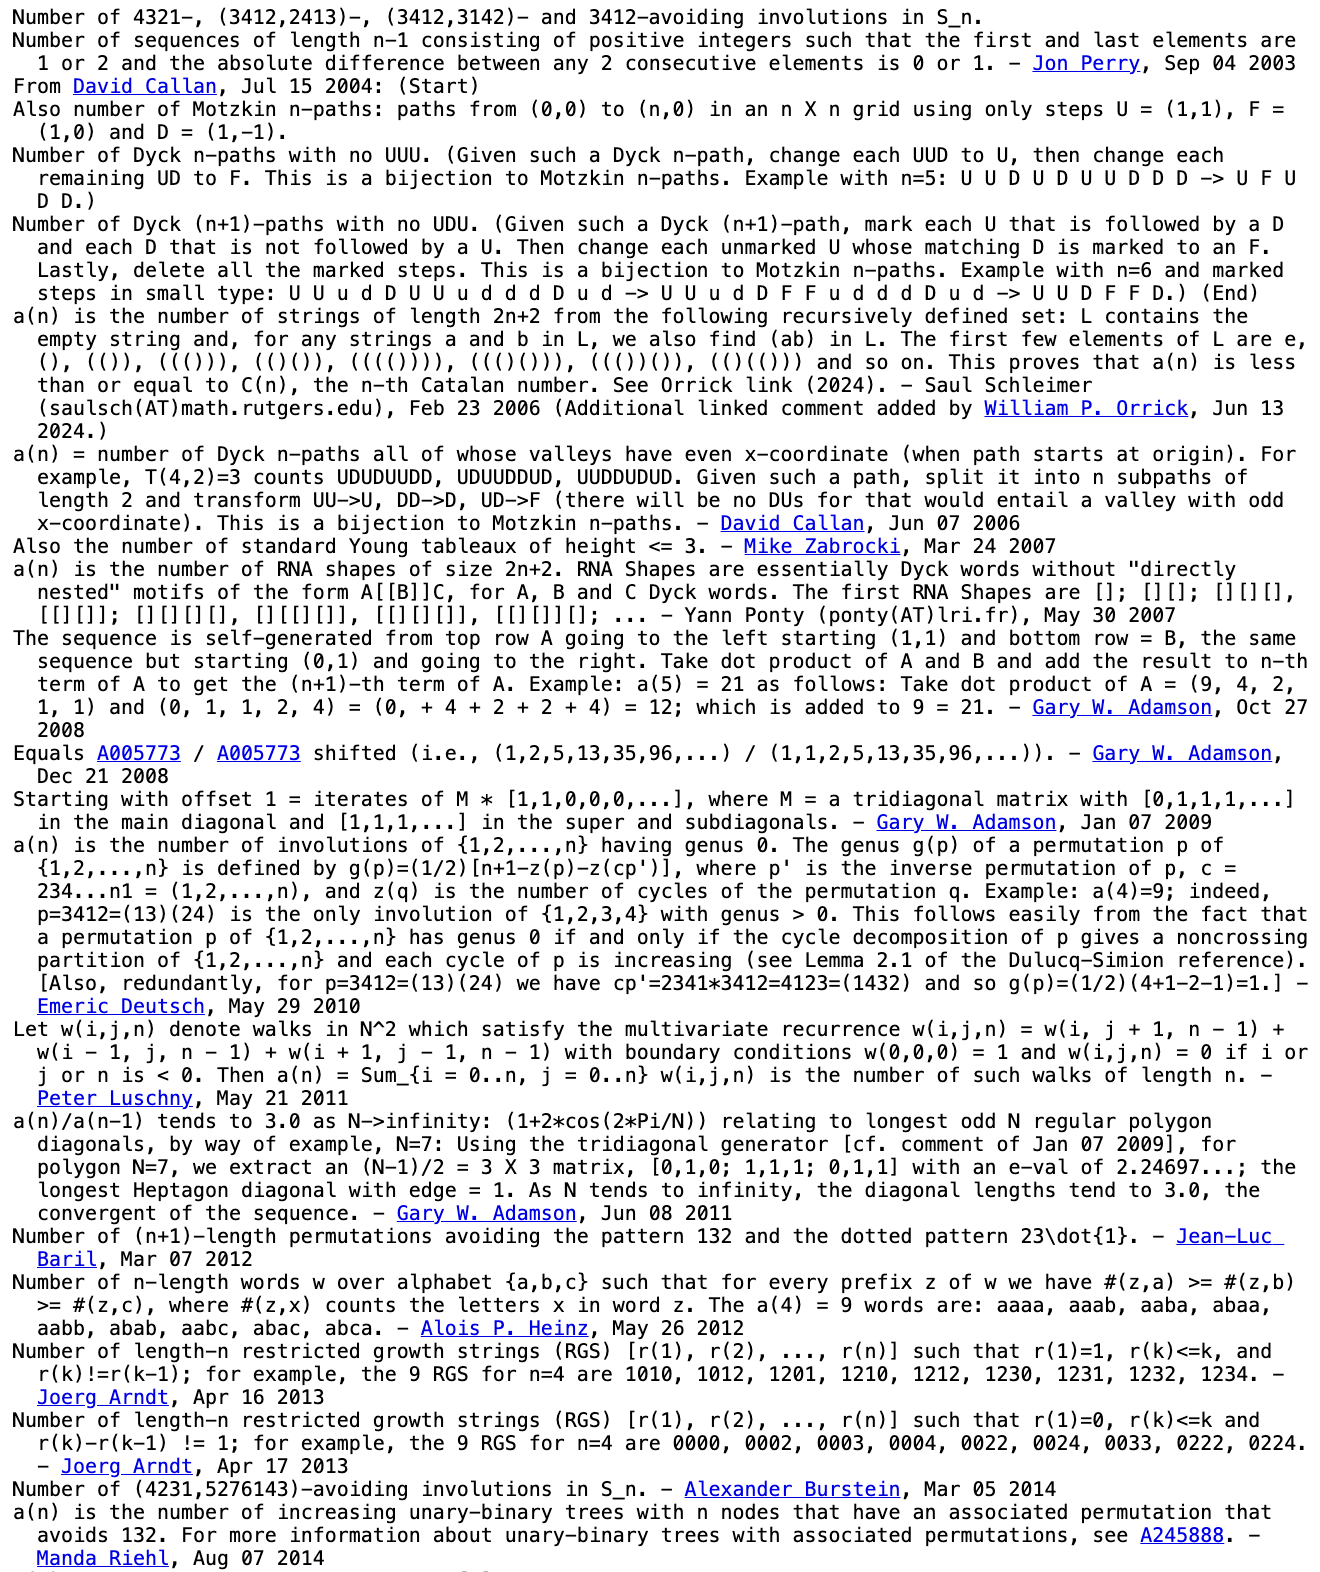
\includegraphics[width=0.49\linewidth]{Images/oeis1.png}
        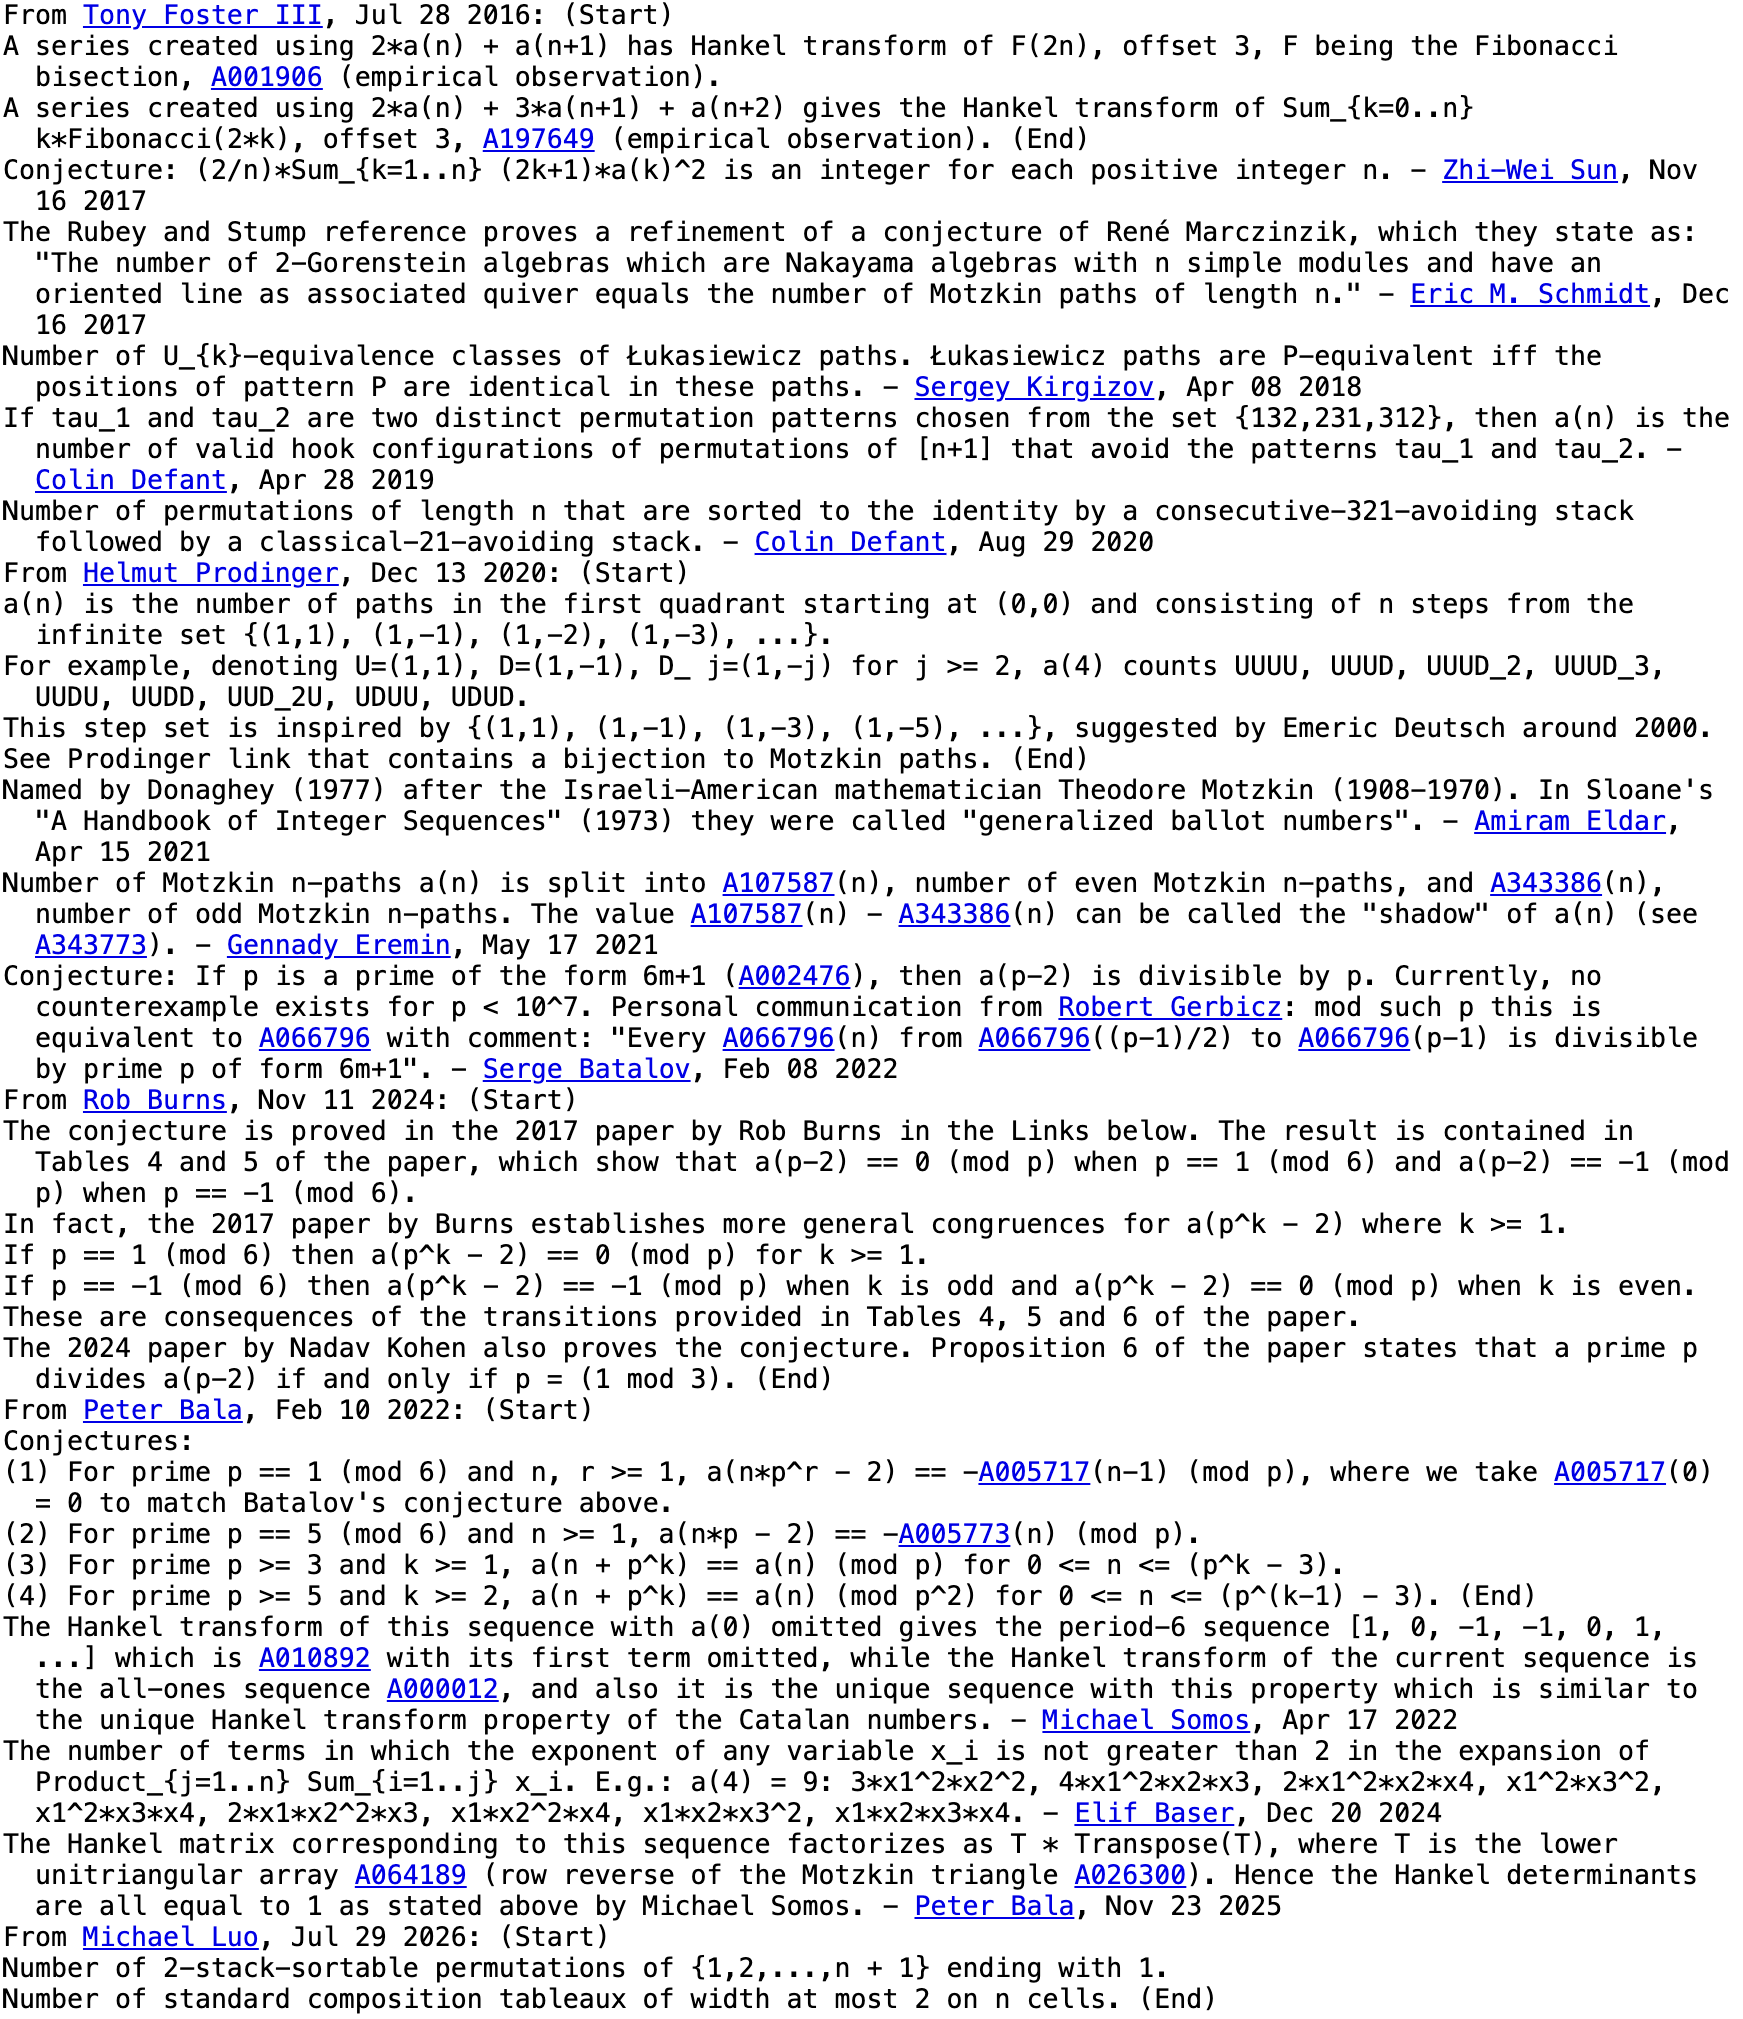
\includegraphics[width=0.49\linewidth]{Images/oeis2.png}
    \end{figure}
    \blfootnote{\tiny Online Encyclopedia of Integer Sequences, August 5, 2026}
    }
    \only<2>{
    $n$th Motzkin counts:
    \begin{figure}
        \centering
        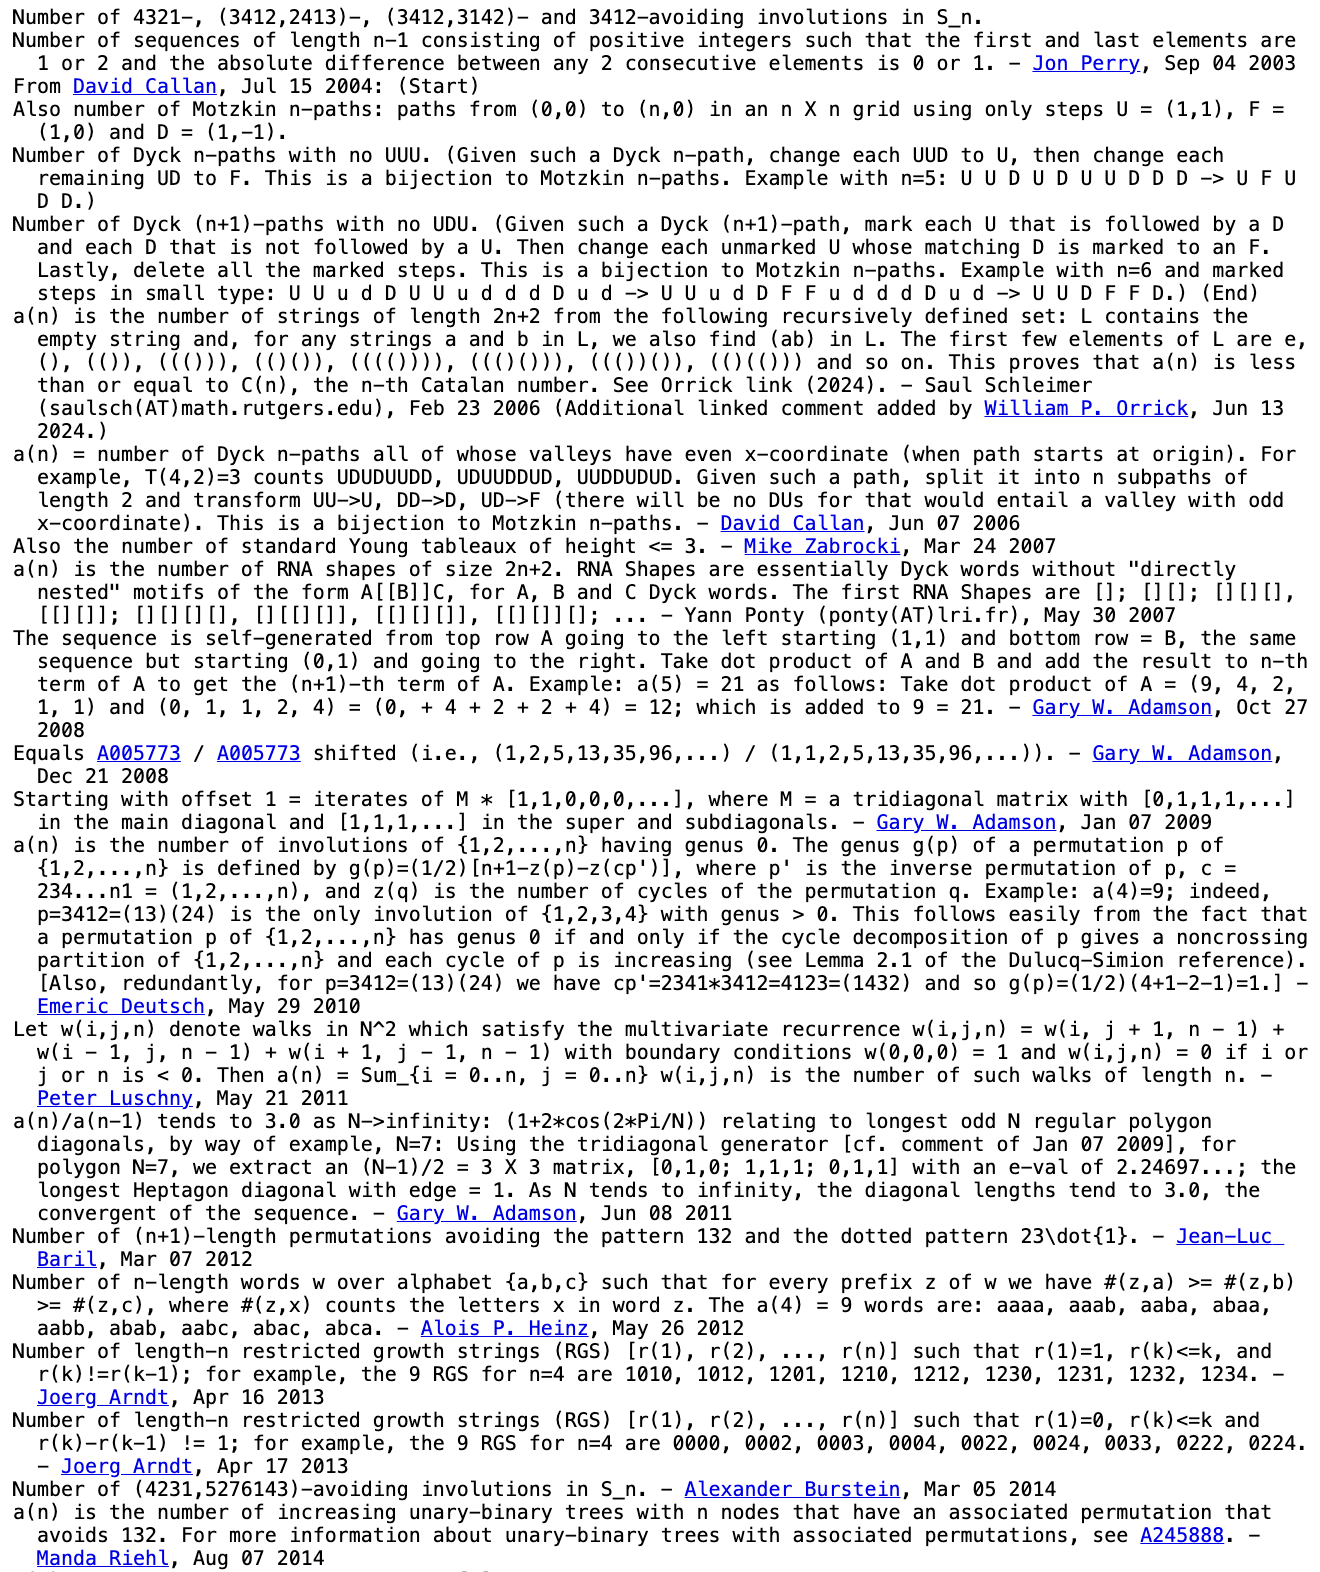
\includegraphics[width=0.49\linewidth]{Images/oeis1.png}
        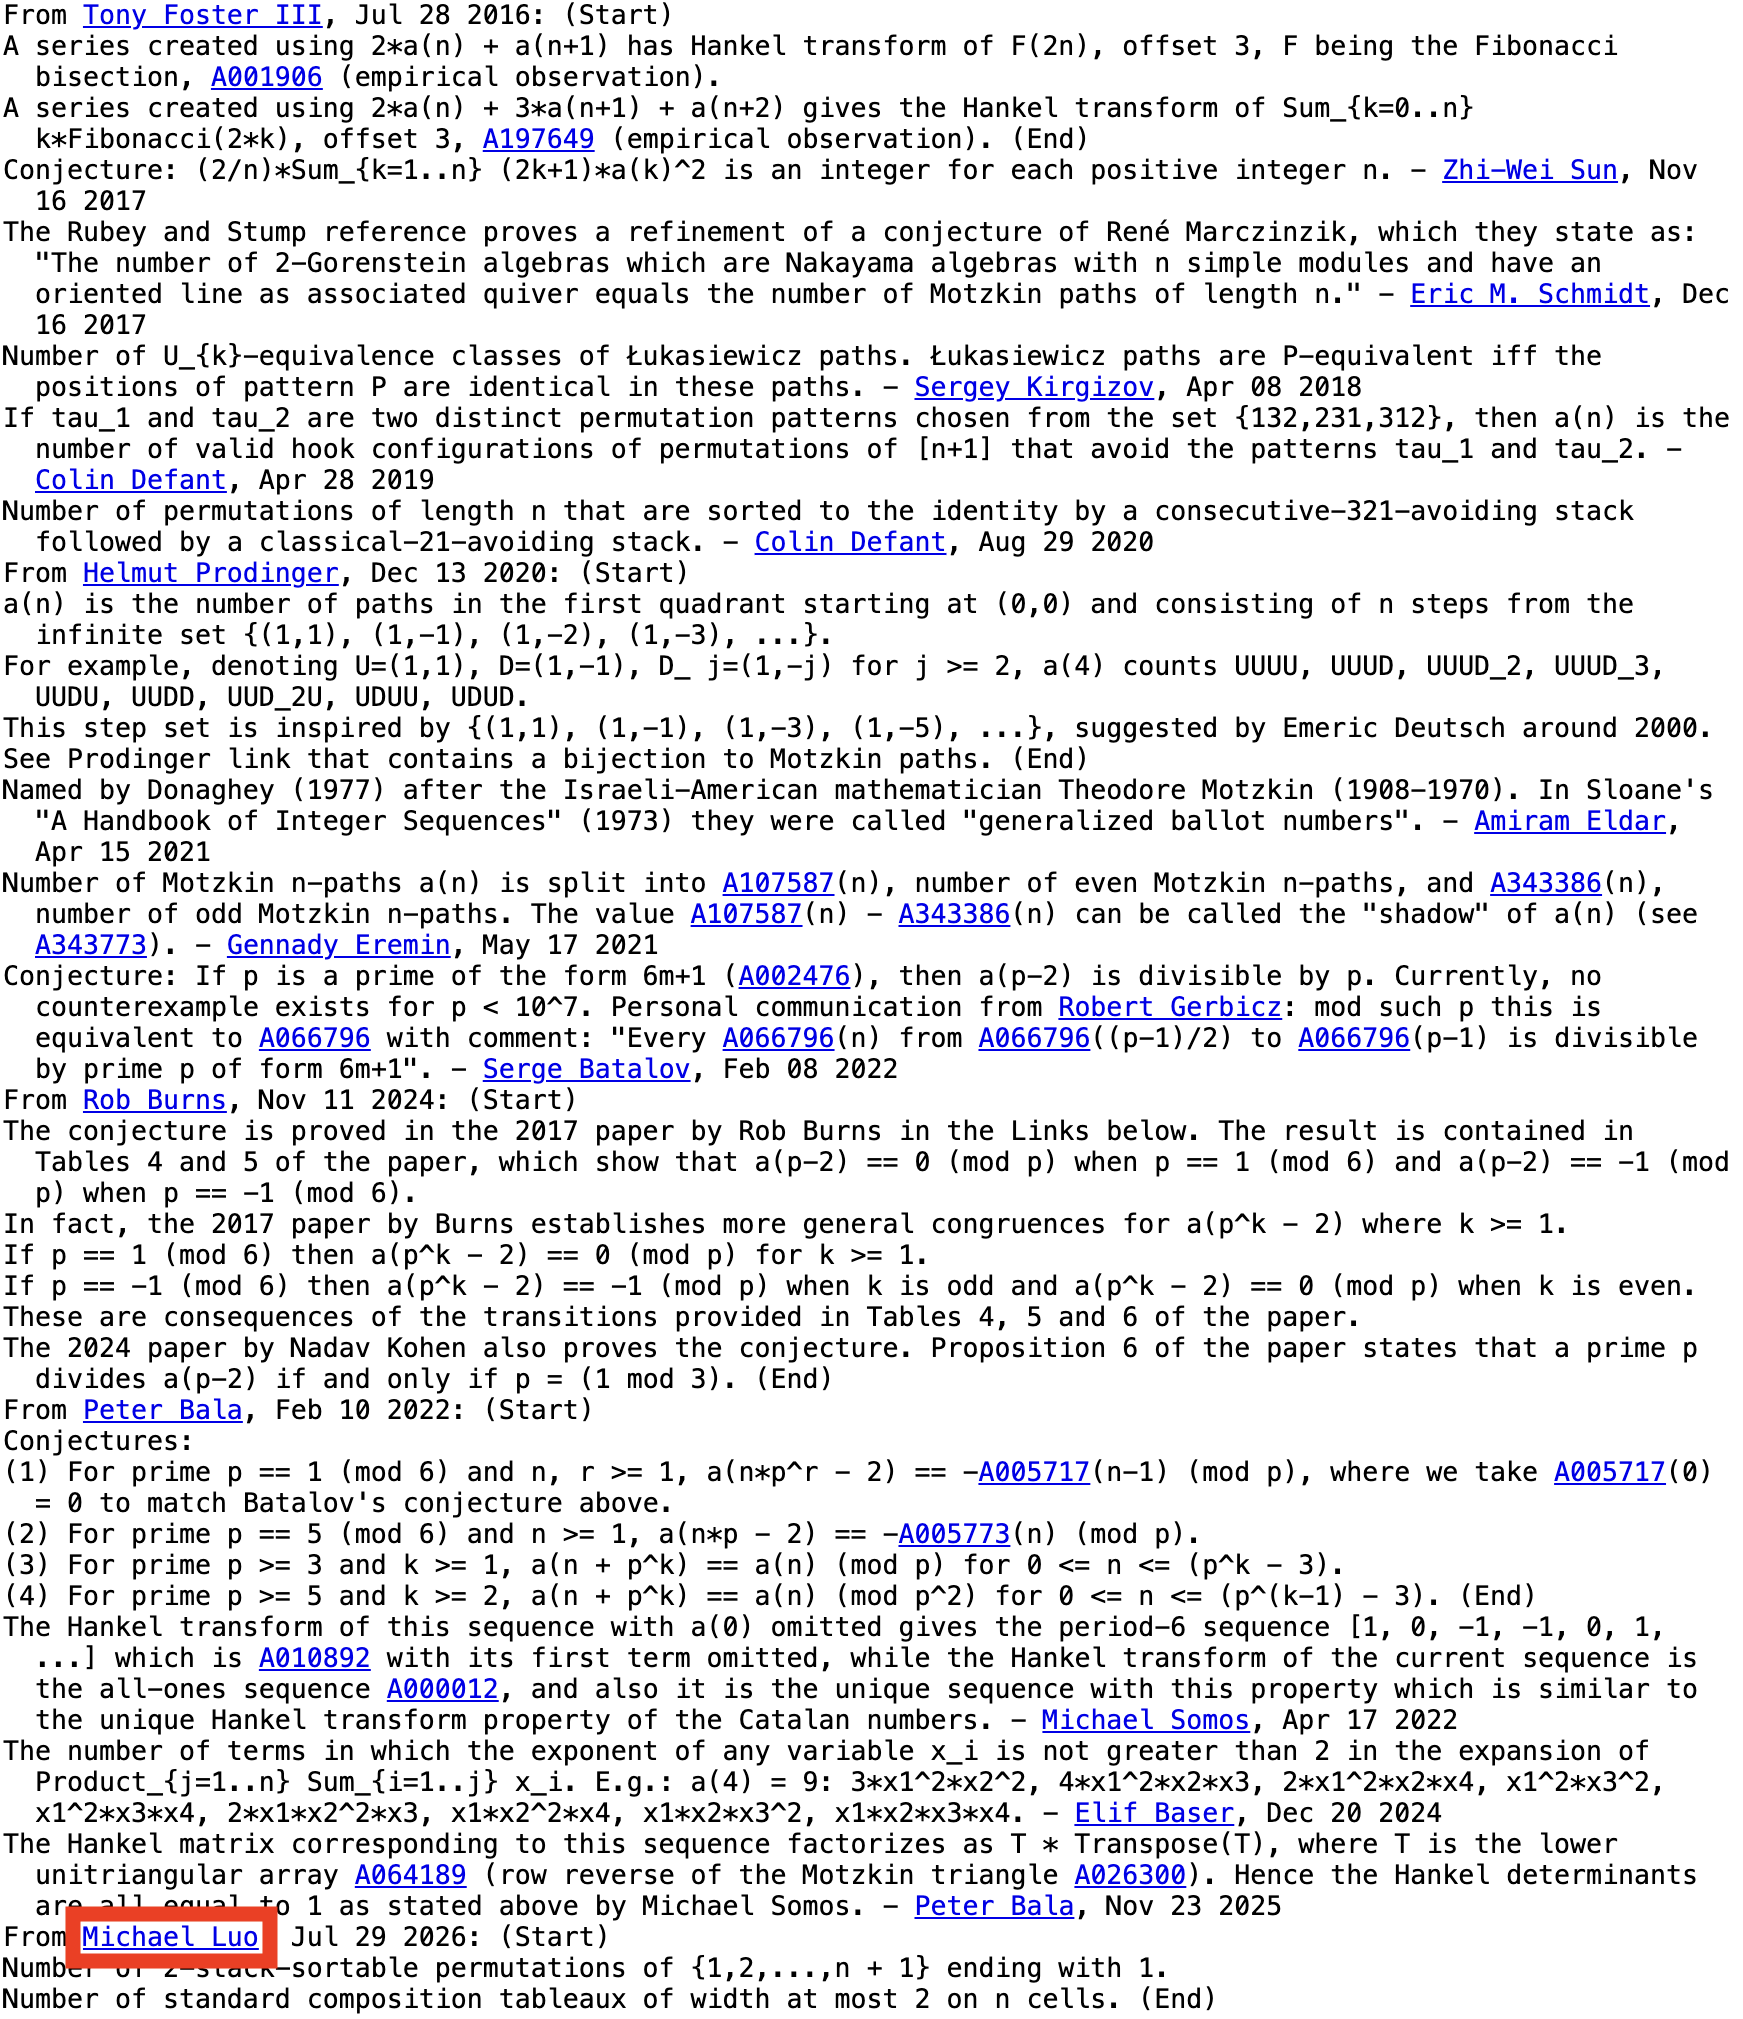
\includegraphics[width=0.49\linewidth]{Images/oeis3.png}
    \end{figure}
    \blfootnote{\tiny Online Encyclopedia of Integer Sequences, August 5, 2026}
    }
    \only<3>{
    \begin{figure}
        \centering
        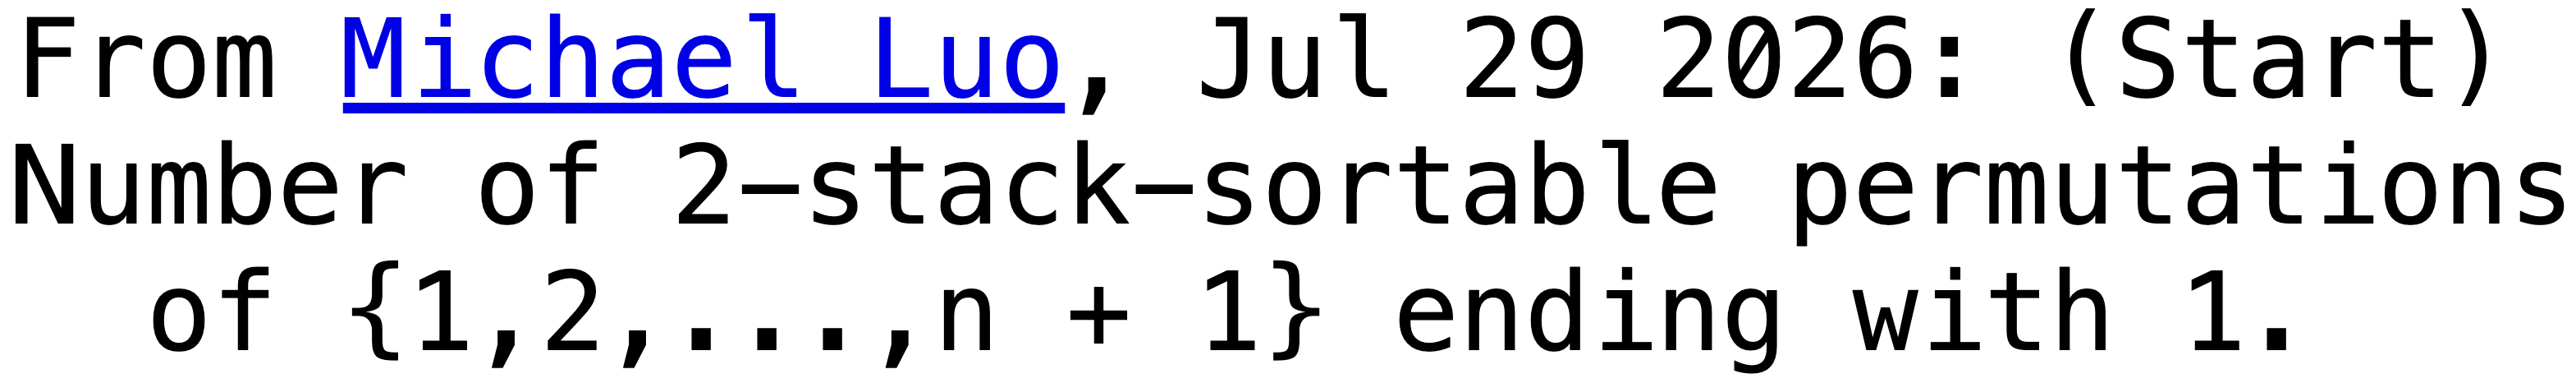
\includegraphics[width=\linewidth]{Images/oeis4.png}
    \end{figure}
    \blfootnote{\tiny Online Encyclopedia of Integer Sequences, August 5, 2026}
    }
\end{frame}

\begin{frame}
    \frametitle{Acknowledgements}
    I thank
    \begin{itemize}
        \ii my mentor Ryota Inagaki
        \ii my tutor AnaMar\'ia Perez
        \ii Tanya Khovanova, David Jerison, Jonathan Bloom
        \ii TAs Jaeho Lee, Frederick Song, Celine Zhang
        \ii Timothy Chen, Xindi Luo, and Sowmya Sankaran
        \ii Colin Defant for help formulating the project
        \ii Jerry Zhang
        \ii MIT and CEE
        \ii my sponsor Joseph Mandarino
    \end{itemize}
\end{frame}

\begin{frame}[plain,noframenumbering]
    \[\text{$s^2$-sortable of $S_n'$} \arw \text{antistandard composition tableaux, width $\le 2$}\]
    \pause\medskip
    \[\text{$s^t$-sortable of $S_n'$} \arw \text{antistandard composition tableaux, width $\le t$}\]
    \pause\medskip
    Applications of $s$ correspond to cutting off columns:
    \[\begin{matrix}
        \text{\LARGE $465213\GRN0$} & \xmapsto s & \text{\LARGE $412\GRN0356$} & \xmapsto s & \text{\LARGE $1\GRN023456$} & \xmapsto s & \text{\LARGE $\GRN0123456$} \\ \\
        \tab{6 & 4 \\ 5 \\ 3 & 2 & 1} & \rightarrow & \tab{4 \\ 2 & 1} & \rightarrow & \tab{1} & \rightarrow & \varepsilon
    \end{matrix}\]
\end{frame}

\begin{frame}[plain,noframenumbering]
    \emph{Power} $p(c)$ of a cell:
    {\Large\[\tab{10 & 9 & 5 \\ *(Salmon) 8 & *(Salmon) 7 \\ *(Salmon) 6 \\ *(Salmon) 4 & *(Salmon) 3 & *(Salmon) 2 & *(Apricot) 1}\]}
    \begin{theorem}[Zhang 2026]
        \# of words in $S_n'$ corresponding to $T$ is
        \[\prod_c p(c),\]
        where product taken over $c \in T$ not in first column.
    \end{theorem}
\end{frame}

\begin{frame}[plain,noframenumbering]
    \begin{theorem}[Zhang 2026]
        The number of $s^t$-sortable permutations in $S_n'$ is computable in polynomial time in $n$.
    \end{theorem}

    \begin{theorem}[Zhang 2026]
        Let $f(n)$ be the average number of iterations needed to sort $\pi \in S_n$. Then $\lim_{n\to\infty}\frac{f(n)}n$ exists.
    \end{theorem}
\end{frame}

\begin{frame}[plain,noframenumbering]
    $s_m$ allows $m$ identical penguins in hole. \only<2->{$s_2$:}
    \only<1>{\invisstack}
    \only<2>{\stack{}{}{}{}{}{212121}}
    \only<3>{\stack{}{}{}{}{2}{12121}}
    \only<4>{\stack{}{}{}{1}{2}{2121}}
    \only<5>{\stack{1}{}{}{}{2}{2121}}
    \only<6>{\stack{1}{}{}{2}{2}{121}}
    \only<7>{\stack{1}{}{1}{2}{2}{21}}
    \only<8>{\stack{11}{}{}{2}{2}{21}}
    \only<9>{\stack{112}{}{}{}{2}{21}}
    \only<10>{\stack{112}{}{}{2}{2}{1}}
    \only<11>{\stack{112}{}{1}{2}{2}{}}
    \only<12>{\stack{1121}{}{}{2}{2}{}}
    \only<13>{\stack{11212}{}{}{}{2}{}}
    \only<14->{\stack{112122}{}{}{}{}{}}
    \uncover<15-16>{$s_7$ ``more powerful'' than $s_6$: every $s_6$-sortable word $s_7$-sortable. }%
    \uncover<16>{But:
    \begin{theorem}[L.\ 2026]
        For all $m \neq m'$, there are words $w$ such that $w$ takes much longer to sort with $s_m$ than $s_{m'}$.
    \end{theorem}
    }
\end{frame}

\end{document}